\chapter{Numerical methods}
\label{app:numerics}

\section*{Integration}
\subsection*{Gauss quadratures}
In order to perform numerical integration we discretise radial and two angles integrals into a quadrature sums \cite{Press:2007:NRE:1403886} as follows:
\beqa
\int d(k^2) \frac{k^2}{2} \int_{-1}^1 dz\sqrt{1-z^2} \int_{-1}^1 dy \longrightarrow \sum^{N_k}_{n=1} \sum^{N_z}_{m=1} \sum^{N_y}_{l=1} w(k_n) w(z_m) w(y_l)\;,
\eeqa
where $w(k_n), w(z_m), w(y_l)$ are quadrature weights and $k_n, z_m, y_l$ are correspondent nodes. The integral over $\phi$ is not considered here since it is for our calculation it is trivial and equal $2\pi$. The radial and $y$-angle integrations involve a trivial integration measure therefore for them we employ Gauss-Legendre quadrature. In case of $z$-angle we need to incorporate the factor $\sqrt{1-z^2}$ into quadrature rule to archive a good accuracy. The proper way to do so is to apply Gauss-Chebyshev quadrature by expanding the integral into following form:
\beqa
	\int_{-1}^1 dz\sqrt{1-z^2} f(z)  \longrightarrow \sum^{N_z}_{m=1} w(z_m) f(z_m)\;,
\eeqa
here nodes are $z_m=cos(\frac{m}{N_z+1}\pi)$ and weights are $w_m=\frac{\pi}{N_z+1}sin^2(\frac{m}{N_z+1}\pi)$. 
%
\subsection*{Cauchy integration}
\begin{figure}[!b]
\begin{center}
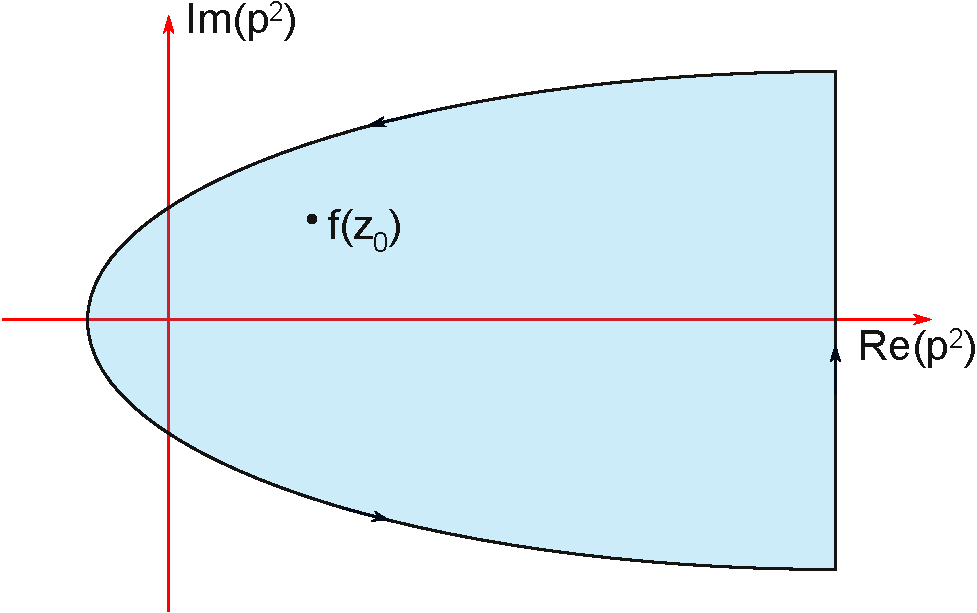
\includegraphics[width=0.8\columnwidth]{figures/contour}
\caption{Sketch of the integration contour for the determination of the quark propagator in
the complex plane.}\label{fig:contour1}
\end{center}
\end{figure}
%
In the BSE due to the external total momentum of the bound state one needs to evaluate the
internal propagators on the right hand side in a parabola region given by Eq.(\ref{dse:contour}) and sketched in Fig.~\ref{fig:contour1}.
Recall that parabolic $p^2$-contour in complex momentum region is parametrizes as follows:
\beqa
	p^2 = t^2 + itM_{state} - \frac{M_{state}^2}{4}\;,
	\label{dse:app_contour}
\eeqa
where the parameter $t$ in given by Gauss quadrature notes $k_n$.
The DSE is then solved iteratively on the boundary supplemented
with Cauchy's theorem, which reads as: given a function $f(z)$ defined on the 
boundary of a closed contour $z\in\mathcal{C}$, we have for any $z_0$ inside:
%
\begin{align}\label{eqn:cauchy}
f(z_0) = \frac{1}{2\pi i} \oint_{\mathcal{C}} \frac{dz f(z)}{z-z_0}\simeq \frac{1}{2\pi i} \sum_{i} \frac{w_i f(z_i)}{z_i-z_0}\;,
\end{align}
%
where the integral has been approximated by some quadrature formula with weights $w_j$ and 
abscissa $z_j$. This is paired with a parametric mapping that describes the contour's boundary.
Numerically this procedure poses a challenge when $z_0$ approaches the abscissa $z_i$. This can be 
mitigated through the use of the barycentric formula~\cite{Berrut_barycentriclagrange}
%
\begin{align}\label{eqn:cauchybary}
f(z_0) = \frac{\sum_{i} \bar{w}_i f(z_i)  }{\sum_{i} \bar{w}_i }\;,\;\;\;\;\bar{w}_i=w_i /\left(z_i-z_0\right)\;
\end{align}
%
%
With this improvement applied, when when $z_0$ approaches the abscissa $z_i$ and the nominator diverges the same happens in denominator so the divergences cancel up to first order error. 

\section*{Power method}
The basic idea is to start with initial guess for the solution and then to generate iterative series converging to the final solution. The scheme can be represented by Eq. \ref{app:solution_scheme}:
\beqa
\label{app:solution_scheme}
F^{(1)}(p) = K(k,p,...) \otimes F^{\text{initial guess}}(k) \\ 
F^{(2)}(p) = K(k,p,...) \otimes F^{(1)}(k) \\ 
\notag &...& \\
F^{(n)}(p) = K(k,p,...) \otimes F^{(n-1)}(k)
\eeqa
Here a number in brackets denote an iteration step, the $K(k,p,...)$ schematically represents the appropriate quark-quark scattering kernel for quark DSE or meson BSE. The sign $\otimes$ represent the the Dirac trace and integration. In this case the sampling of the internal grid $(k)$ can be set similar to external grid $(p)$. Note that the quark DSE takes as input the quark propagator $S(k)$, but outputs inverted one $S^{-1}(p)$. The iterations must be performed until they converged to solution at desired accuracy level.  \\ 

In case of shifted momenta, as it was considered in \ref{chap:BSE}, this robust method cannot be applied due to non-trivial momenta routing:
\beqa
F(p) = K_{\text{shifted}}(k,p,...) \otimes F(p-k)\;, 
\label{app:solution_scheme_shift1}
\eeqa
where a notion $\text{shifted}$ reflects the fact that the scattering kernel also changes due to the momenta shifting. From Eq.(\ref{app:solution_scheme_shift1}) it is clear, that the internal grid $(p-k)$ does not match to external $(p)$ and moreover the internal grid depends on external. The additional complexity comes from the fact that in case of quark DSE the propagator, meant to be used in meson BSE later, has to be obtained within parabolic region in complex plane defined by:
\beqa
	p^2 = t^2 + itM_{meson} - \frac{M_{meson}^2}{4} 
	\label{app:contour}
\eeqa
The following external grid $(p^2)$ and internal grid $(p-k)^2$ are shown on Fig. \ref{fig:contour2}. 
\begin{figure}[h]
\begin{center}
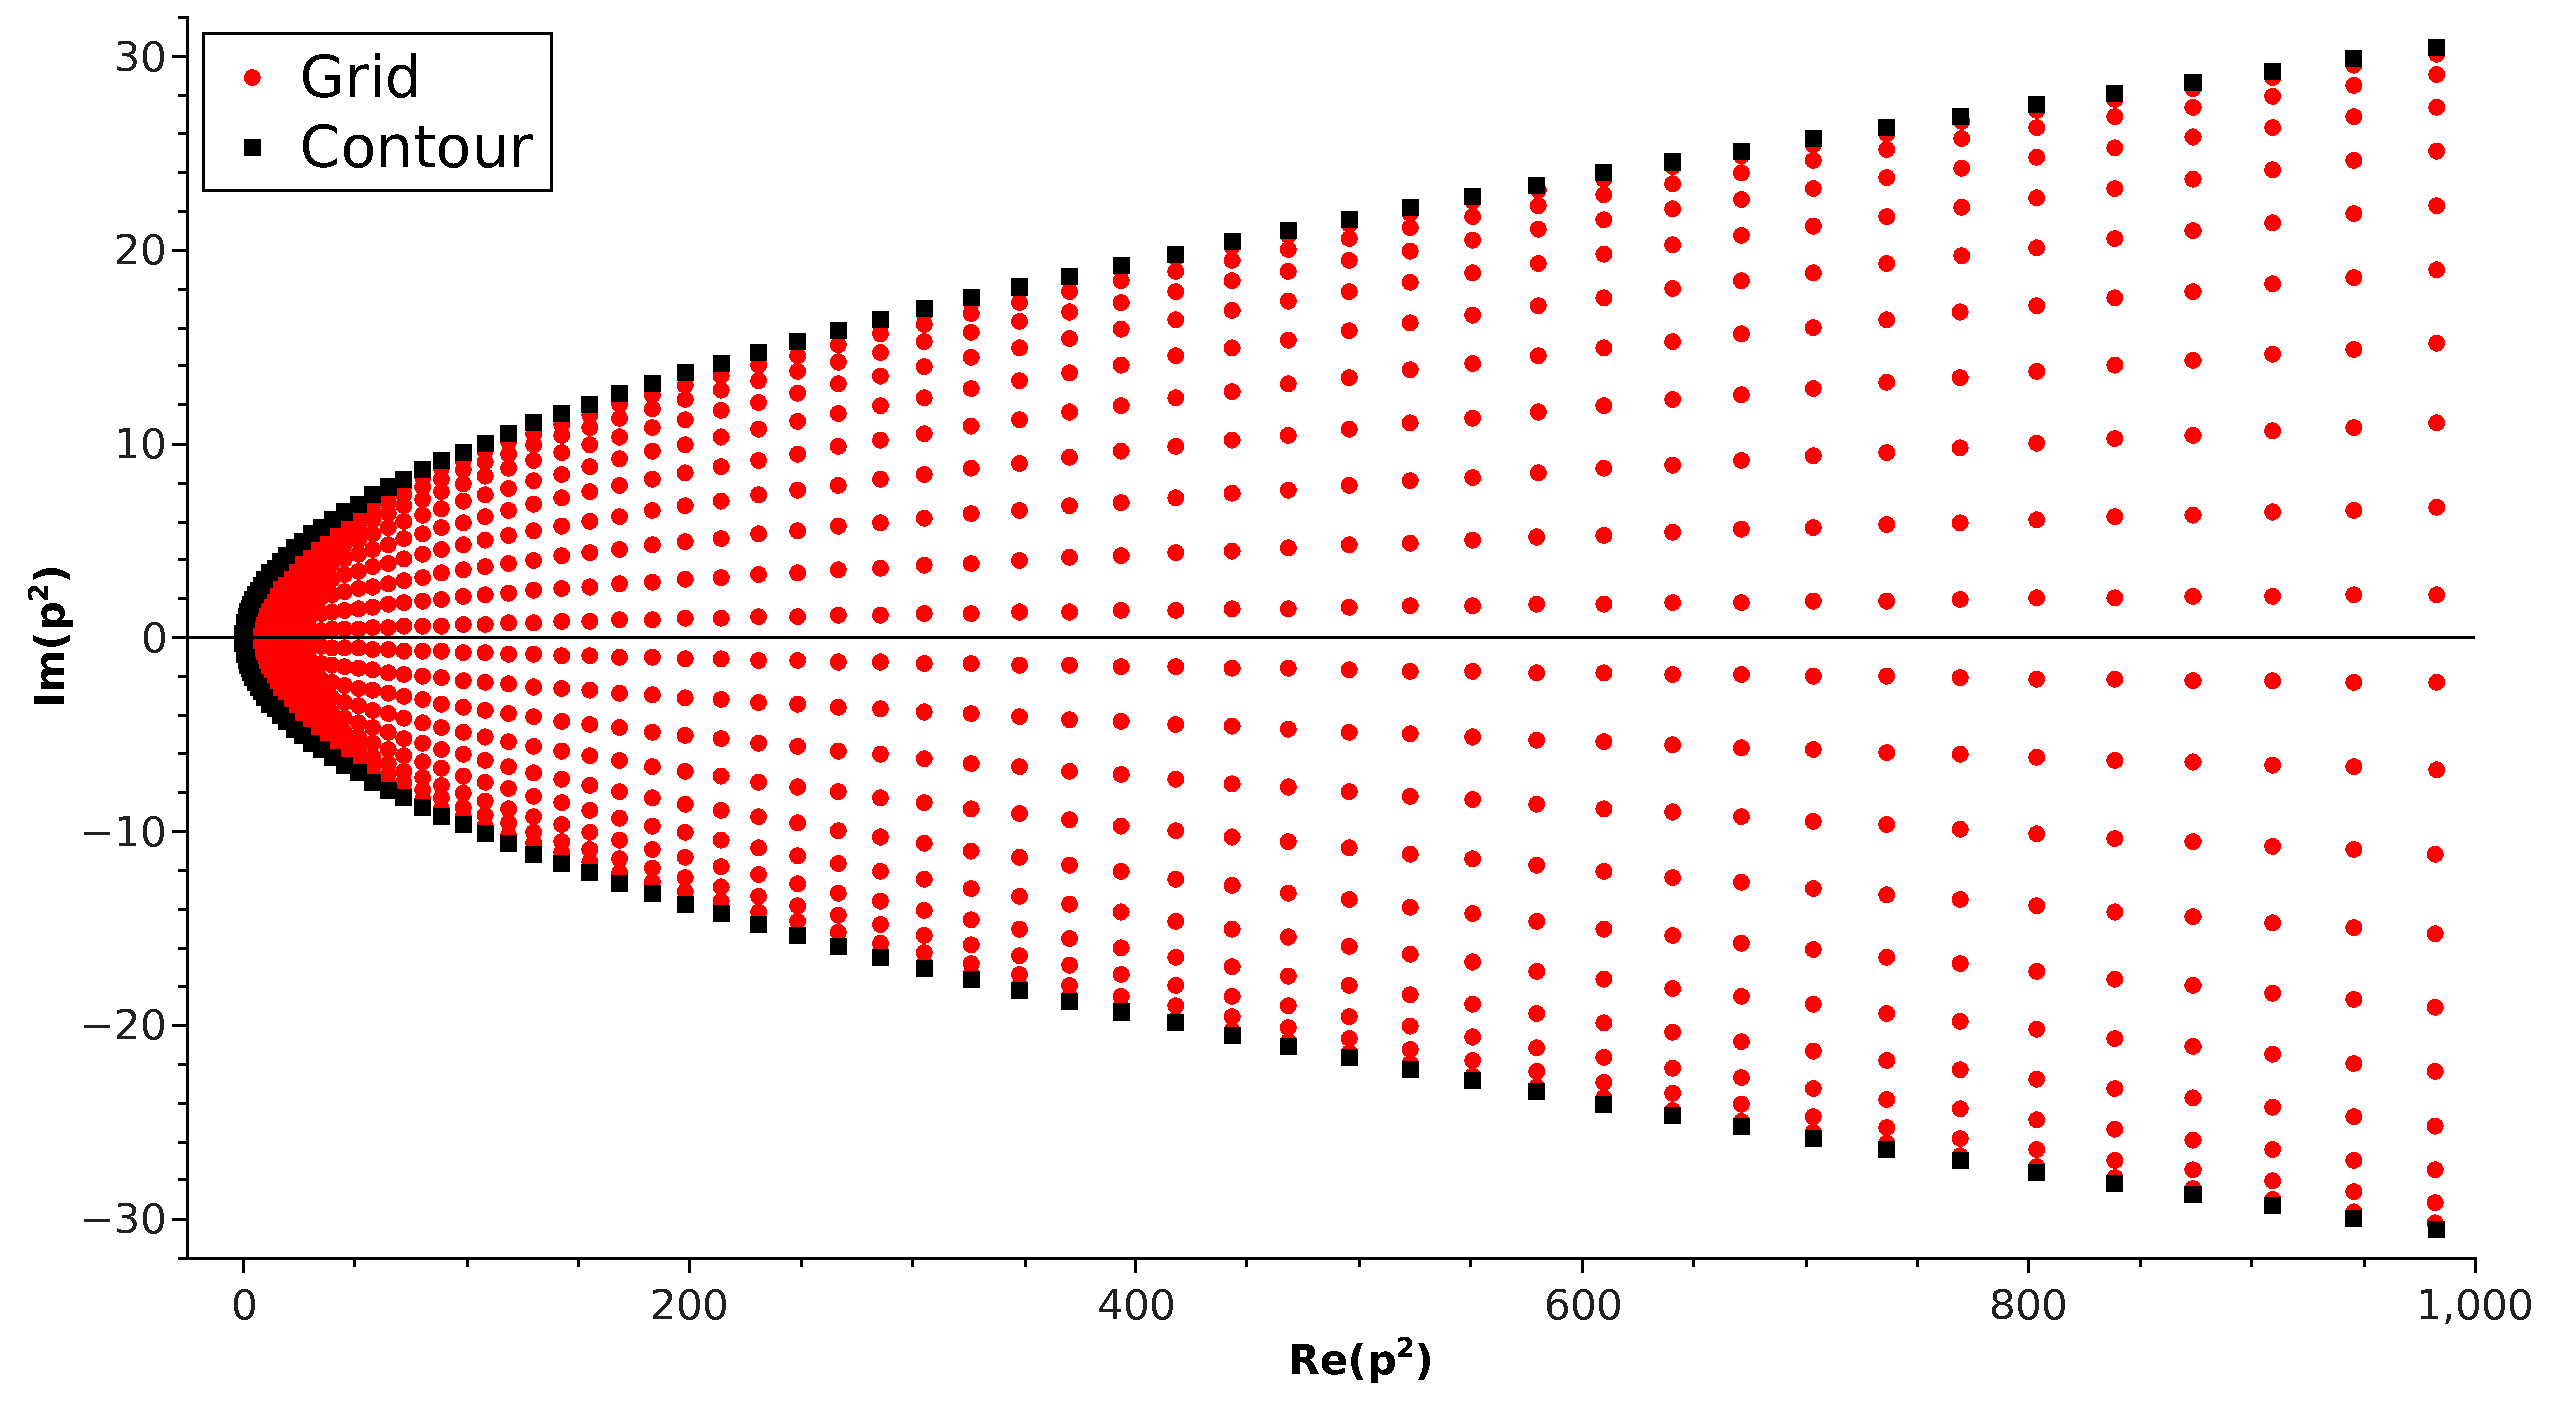
\includegraphics[width=0.99\textwidth]{figures/Grid_to_Contour}
\caption{\footnotesize }\label{fig:contour2}
\end{center}
\end{figure}
However the two observations can be made: every point of the internal grid $(p-k)^2$ for any $k$ lies within parabolic region $(p^2)$; the dressing functions posses analyticity property and therefore if they are known on a contour, using the Cauchy theorem we can obtain them everywhere inside a contour. In order to employ this idea we need to truncate our parabolic region at $\Lambda$ UV scale and by that turn it into the contour, where $\Lambda$ is same as the upper limit of a loop integration. The power method in this case has one extra step:
\beqa
\label{app:solution_scheme_shift2}
F^{(1)}(p) = K_{\text{shifted}}(k,p,...) \otimes F^{\text{initial guess}}(p-k) \\
F^{(1)}(p-k) = \mathfrak{C} \left(  F^{(1)}(p) \right)  \\ 
F^{(2)}(p) = K_{\text{shifted}}(k,p,...) \otimes F^{(1)}(p-k) \\
\notag &...& \\
F^{(n)}(p) = K_{\text{shifted}}(k,p,...) \otimes F^{(n-1)}(p-k)\;,
\eeqa
here $\mathfrak{C}$ denotes the mapping from external grid $(p^2)$ to internal grid $(p-k)^2$ via the Cauchy integral. The Eq.(\ref{app:solution_scheme_shift2}) is written in a general notation to stress the fact that this approach can be applied to both quark DSE and homogeneous/inhomogeneous meson BSE. The power methods have a major drawback - one can obtain only the first dominant solution and in case of meson BSE this would mean it would obtain only the ground state. 

\section*{Matrix eigenvalue calculation}
The meson \BSE can be considered as eigenvalue problem, such that the Eq.(\ref{bse:BSE_gen}), given by:
\beqa
	\Gamma^{(\mu...)}_{tu}(p;P) = \lambda(P^2) \int \frac{d^4 k}{(2\pi)^4} K_{tu;rs}(p,k;P)\left[ S(k_+)\Gamma^{(\mu...)}(k;P)S(k_-)\right]_{sr}\;,
	\label{app:BSE_gen}
\eeqa
after transforming the integration into Gaussian quadrature \cite{Press:2007:NRE:1403886} according to Appendix \ref{app:euclidean}, the meson BSE can be written as:
\beqa
	\mathcal{A}_i = \lambda(P^2) \mathcal{K}_{ik} \mathcal{A}_k\;,
\eeqa
where the index $i$ at $A$ denotes not only the appropriate scalar \BS amplitude but also the quadrature integration point, so the vector $A_i$ takes the following form:
\beqa
\mathcal{A} =
	\begin{pmatrix} 
A_1(p^2_{(1)},z_{(1)},P^2) \\
A_1(p^2_{(2)},z_{(1)},P^2) \\
... \\
A_1(p^2_{(1)},z_(2),P^2) \\
... \\
A_2(p^2_{(1)},z_{(1)},P^2) \\
...
\end{pmatrix},
\eeqa
and the matrix $\mathcal{K}_{ik}$ consists of traces of the angular tensor in $\Gamma^{(\mu...)}_{tu}(p;P)$ from r.h.s in Eq.(\ref{bse:BSE_gen}), the scattering kernel $K_{tu;rs}(p,k;P)$, two propagators $S(k_+),S(k_-)$ and the the angular tensor in $\Gamma^{(\mu...)}(k;P)$ from l.h.s, so the matrix $\mathcal{K}_{ik}$ reads as:
\beqa
Tr \left[  D^{(i)}_{r}(p^2_{(i)},z_{r(i)}) K(p^2_{(i)},z_{r(i)},k^2_{(k)},z_{l(k)})  S_+(k^2_{(k)}) D^{(k)}_{l}(k^2_{(k)},z_{l(k)}) S_-(k^2_{(k)}) \right],
\eeqa
where $D_{r}(p;P)$ and $D_{l}(k;P)$ are the angular tensors from r.h.s and l.h.s respectively and for a brevity we omitted $P$ dependence. In simple words the index $i$ denotes iteration over amplitude projector $D_{r}$ and over $(p^2,z_r)$ external grid points, whether index $k$ denotes amplitude projector $D_{r}$ and $(k^2,z_l)$ internal grid points. Once the matrix $\mathcal{K}_{ik}$ in allocated on the required external $(p^2,z_r)$ and internal $(k^2,z_l)$ grids for all amplitudes for the desired $J^{PC}$ we can employ the numerical eigenvalue calculation routine, namely the eigenvalue decomposition. The numerical routine is provided by the \emph{Eigen} library~\cite{eigenweb}. We specify the $J^P$ of the state through the choice of the covariant decomposition, section~\ref{bse:angular_tensor}, and determine the $C$-parity of the state by examining the symmetry properties of the eigenvector. \\